\documentclass{beamer}

\usetheme{MagdeburgFIN}
\usefonttheme{structurebold}
\usepackage{graphicx}
\usepackage{float}
\usepackage{url}
\usepackage{pdfpages}
\usepackage{xfrac}
\usepackage[export]{adjustbox}
\usepackage{wrapfig}
\usepackage{verbatim}

\setbeamertemplate{caption}[numbered]

\title{MS-III. Implementation}
\author{Ali Hashaam, Ali Memon, Guzel Mussilova, Pavlo Shevchenko}
\date{June 13, 2017}
\institute{Scientific Project: Databases for Multi-Dimensional Data, Genomics and Modern Hardware}

\begin{document}

\begin{frame}[plain]
 \titlepage
\end{frame}

\begin{frame}
\frametitle{Table of Contents}
\tableofcontents 
\end{frame}

\section{Blinktopus}
\begin{frame}
\frametitle{Our Goal}
To provide a \textbf{framework} that gives user a chance to act as \textit{Holistic SV Optimizer} like in OctopusDB \\
Add \textbf{Approximate Query Processing (AQP)} techniques\\
\textbf{Evaluate} performance depending on choice of SV
\end{frame}


\section{Recall}
\begin{frame}
\frametitle{Building a Blinktopus. Recall}
First, the Octopus:
\begin{itemize}
\item{Store incoming data in logs.}
\item{Query the logs (just a filter query).}
\item{Allow users to create views (row, column) over certain logs.}
\item{List all views and logs.}
\item{Launch the query over views or over logs, see the changes in performance.}
\end{itemize}
\end{frame}


\begin{frame}
\frametitle{Building a Blinktopus. Recall}
Enters Approximate Query Processing (AQP):
\begin{itemize}
\item{Which synopsis will we choose to test? (Samples, histograms, sketches?)}
\item{Do Octopuses and AQP match well together?}
\item{Build the selected synopsis on the whole data, after data insertions.}
\item{Using the synopsis, answer the user queries by reconstructing the approximate data.}\\
\end{itemize}
\end{frame}


\section{Implementation}

\begin{frame}
%\frametitle{Building a Blinktopus. Implementation}
\hspace{0.2 cm} \textbf{\fontsize{14}{12}\selectfont Building a Blinktopus. Implementation}
\end{frame}

\begin{frame}
\frametitle{Building a Blinktopus. IDE}
\begin{itemize}
\item{Back end}
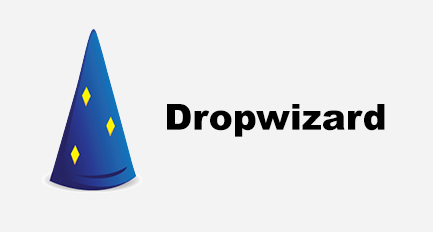
\includegraphics[scale=0.3]{img/dropwizard.png}
\vspace{0.25 cm}
\item{Front end}

\includegraphics[scale=0.2]{img/jpnotebook.png}
\footnote{\tiny 
Sources: http://jupyter.org/\\
http://honstain.com/new-dropwizard-1-0-5-java-service/}
\end{itemize}
\end{frame}

\subsection{Schema}
\begin{frame}
\frametitle{Schema}
\begin{figure}
\centering
\begin{minipage}{.5\textwidth}
 \fontsize{10}{10}\selectfont Selectivity Factors = 1,5,10,15 \\
 \vspace{0.2cm}SF 1 = 1.2 M Records
\end{minipage}%
\begin{minipage}{.5\textwidth}
  \centering
  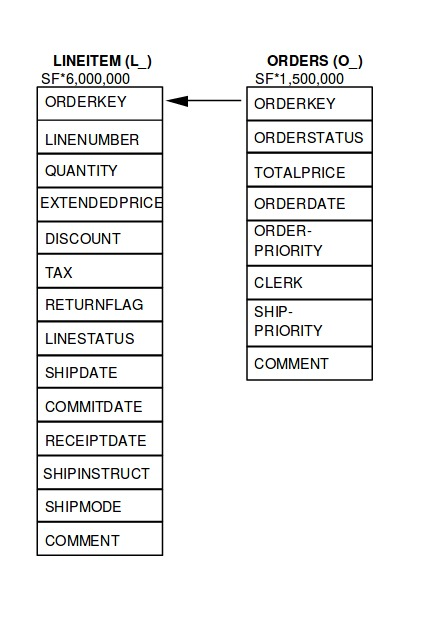
\includegraphics[scale=0.33]{img/Blinktopus-Schema.jpg}
  \caption{\fontsize{6}{5}\selectfont TPC Standard Schema}
\end{minipage}
\end{figure}
\end{frame}


\subsection{OctopusDB}
\begin{frame}
\frametitle{OctopusDB. Customization}
\begin{figure}
\centering
\begin{minipage}{.5\textwidth}
  \centering
  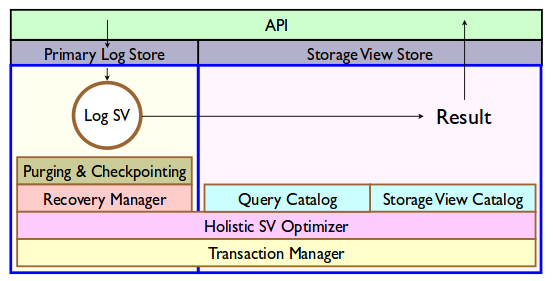
\includegraphics[scale=0.25]{img/octopus_arch.png}
  \caption{\fontsize{8}{5}\selectfont OctopusDB Architecture.}
\end{minipage}%
\pause
\begin{minipage}{.5\textwidth}
  \centering
  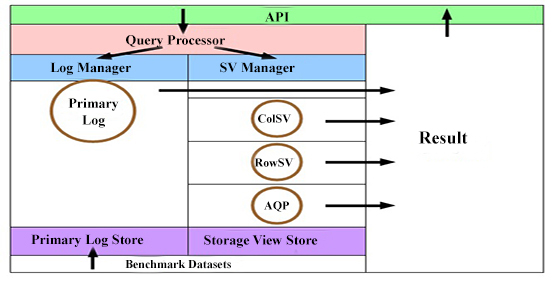
\includegraphics[scale=0.25]{img/Blinktopus-OctopusPart.jpg}
	\caption{\fontsize{8}{5}\selectfont Blinktopus.}
\end{minipage}
\end{figure}
\footnote{\fontsize{5}{5}\selectfont A. Jindal. The Mimicking Octopus: Towards a one-size-fits-all Database Architecture, 2010}
\end{frame}

\begin{frame}
\frametitle{OctopusDB. Evaluation}
\begin{figure}
\centering
\begin{minipage}{.5\textwidth}
  \centering
  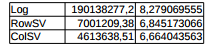
\includegraphics[scale=0.6]{img/Blinktopus-Evaluations3.png}
\end{minipage}
\begin{minipage}{.5\textwidth}
  \centering
  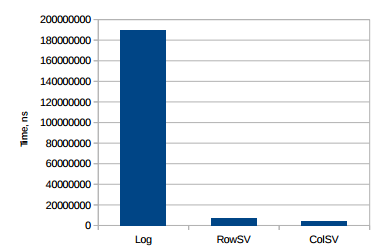
\includegraphics[scale=0.5]{img/Blinktopus-Evaluations1.png}
  \caption{\fontsize{6}{5}\selectfont Storage View Type.}
\end{minipage}%
\begin{minipage}{.5\textwidth}
  \centering
  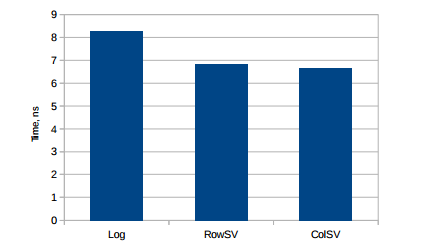
\includegraphics[scale=0.5]{img/Blinktopus-Evaluations2.png}
  \caption{\fontsize{6}{5}\selectfont Storage View Type (Log Scale).}
\end{minipage}
\end{figure}
\fontsize{10}{5}\selectfont Evaluation result for 100 runs over Totalprice Column in Orders with Range from 50,000 to 200,000.
\end{frame}


\subsection{Approximate Query Processing}
\begin{frame}
\frametitle{AQP. Synopses}
4 main families of synopses\footnote{\tiny Cormode, Graham, Minos Garofalakis, Peter J. Haas, and Chris Jermaine. "Synopses for massive data:
Samples, histograms, wavelets, sketches." Foundations and Trends in Databases 4, no. 1–3 (2012): 1-294.}:
\begin{itemize}
\vspace{0.3 cm}
\item{Samples}
\item{Histograms \checkmark}
\item{Wavelets}
\item{Sketches \checkmark}
\end{itemize}
\end{frame}
\subsubsection{Histograms}
\begin{frame}
\frametitle{AQP. Histograms}
	In histogram's development, main cornerstones are:
	\begin{itemize}
		\item {Partition the dataset into buckets.\\Number of buckets 'k':
	\hspace{0.2 cm} $k = 2n^{\sfrac{1}{3}}$ \hspace{0.3 cm} (RICE RULE)}
		\item {Store summary statistics for each bucket about the data values in the it.}
		\item {Store information about the buckets themselves, like bucket boundaries.}
	\end{itemize}
	At query time, the summary and bucket information is used to approximately answer the query.
\end{frame}

\begin{frame}
\frametitle{AQP. Histograms}
	Vital Points to consider:
	\begin{itemize}
		\item Bucketing Scheme
		\item Statistics Stored per Bucket
		\item Approximation Scheme
		\item Class of queries answered		
		\item Efficiency
		\item Accuracy \& Error Estimates
		\item Incremental Maintenance
	\end{itemize}
\end{frame}

\begin{frame}
\frametitle{AQP. Histograms}
\fontsize{10}{5}\selectfont D = \{1.61,1.72,2.23,2.33,2.71,2.90,3.41,4.21,4.70,4.82,4.85,4.91\}
\begin{figure}
  \centering
  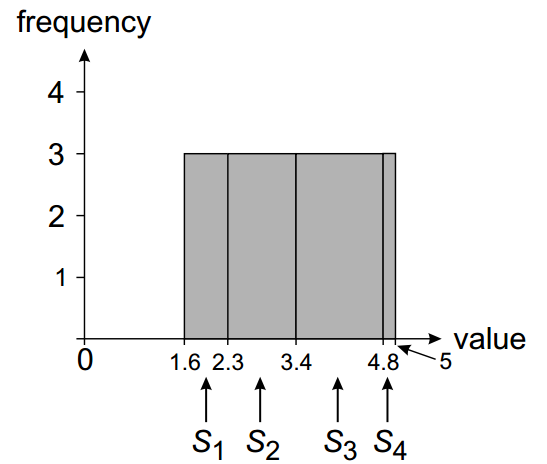
\includegraphics[scale=0.3]{img/Blinktopus-EquiDepth.png}
  \caption{Equi-Depth Histogram \footnote{\fontsize{3}{5}\selectfont Cormode, Graham, Minos Garofalakis, Peter J. Haas, and Chris Jermaine. "Synopses for massive data: Samples, histograms, wavelets, sketches."}}
\end{figure}
What if the count of the values between 1.1 and 4.5 is required?
\end{frame}

\begin{frame}
\frametitle{AQP. Histograms}
Continuous value assumption allows the estimation of values inside a bucket via interpolation.
\begin{figure}
  \centering
  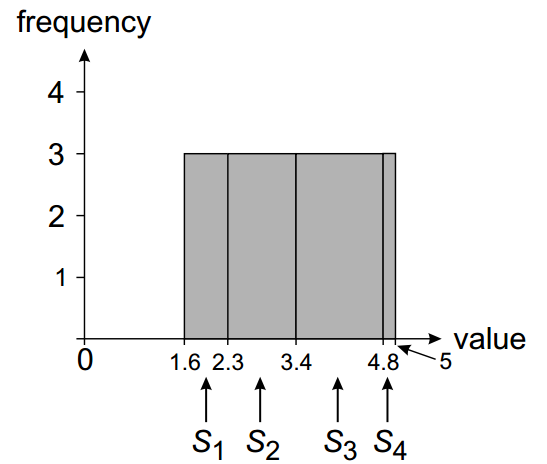
\includegraphics[scale=0.30]{img/Blinktopus-EquiDepth.png}
\end{figure}
Actual query : N = 8\\
$ AQP: N = 3 + 3 + ((4.5 − 3.4)/(4.8 − 3.4))3 = 8.4$\\
Overestimation Error = 5%
\end{frame}

\subsubsection{Sketches}
\begin{frame}
\frametitle{AQP. Sketches}
\begin{itemize}
		\item{Sketches, approximately answer queries by creating small summary data structures that approximately resemble the original data.}
		\item{Appropriate in scenarios involving streaming of big data or analysis of higher dimensional data is required.}
		\item{Other synopsis (Samples, histograms, Wavelets) can be extracted from it.}
\end{itemize}

\end{frame}

\begin{frame}
\frametitle{AQP. Sketches}
Phases of Sketching mechanism:
\begin{figure}
  \centering
  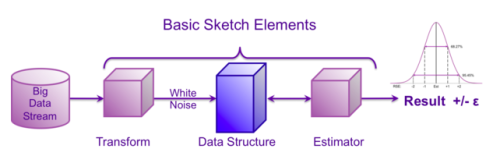
\includegraphics[scale=0.30]{img/distinct_count_sketches.png}
  \caption{Sketching Phases \footnote{\fontsize{3}{5}\selectfont Source: https://yahooeng.tumblr.com/post/135390948446/data-sketches}}
  \end{figure}
  Case Under Scrutiny: Count-Distinct
\end{frame}

\begin{frame}
\frametitle{AQP. HyperLogLog (HLL)}
HLL algorithm estimates the number of distinct elements in large datasets i.e. cardinality, in a single pass, and using a very small amount of memory.\footnote{\fontsize{3}{5}\selectfont Flajolet, Philippe, et al. "Understanding the HyperLogLog: a Near-Optimal Cardinality Estimation Algorithm."}\\
\vspace{0.2cm}
4 billion distinct elements = ${\log_2{\log_2(2^{32})}}$ = 5 bits required 
\end{frame}

\begin{frame}
\frametitle{AQP. HyperLogLog (HLL)}
\begin{figure}
  \centering
  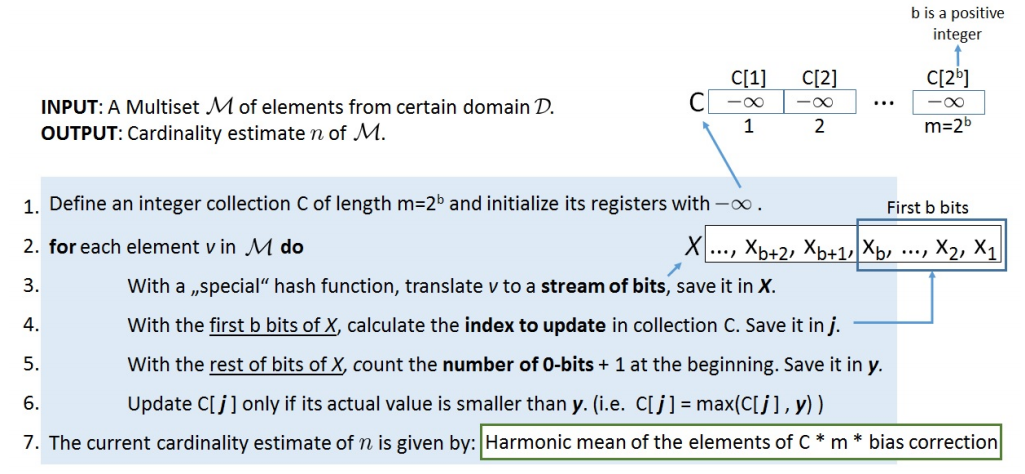
\includegraphics[scale=0.38]{img/HLL.png}
  \caption{ The HyperLogLog algorithm \footnote{\fontsize{3}{5}\selectfont Flajolet, Philippe, et al. "Understanding the HyperLogLog: a Near-Optimal Cardinality Estimation Algorithm."}}
  \end{figure}
\end{frame}

\begin{frame}
\frametitle{AQP. HyperLogLog (HLL)}
\begin{itemize}
	\item{Divide the n distinct elements of the input multiset into m number of buckets.}
	\item{Each bucket must comprises approximately the same number of elements, $\frac{n}{m}$.}
	\item{transform our input multiset M into an ideal multiset via a special Hash function.}
	\item{Hash function will transform the values to a stream of 0’s and 1’s,}
\end{itemize}
\end{frame}

\begin{frame}
\frametitle{AQP. HyperLogLog (HLL)}
\begin{itemize}
	\item{Take first b bits of the hashed value as the index of the bucket.}
	\item{In each bucket only save the longest run of starting 0-bits+1 among all the hashed values of the elements that belong to that bucket.}
	\end{itemize}
	\hspace{0.2cm}n = length of longest run of starting 0-bits + 1\\
	\vspace{0.2cm}
	\hspace{0.2cm}Number of distinct elements in bucket = $2^{n}$\\
	\vspace{0.2cm}
	\hspace{0.2cm}bits required = ${\log_2{\log_2(2^{n})}}$ 
\end{frame}

\begin{frame}
\frametitle{AQP. HyperLogLog (HLL)}
\begin{figure}
  \centering
  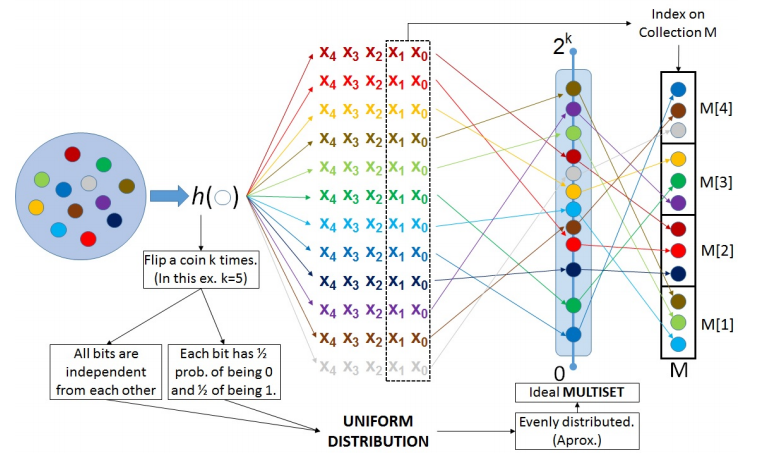
\includegraphics[scale=0.38]{img/HLL2.png}
  \caption{ Randomization of elements and division in buckets \footnote{\fontsize{3}{5}\selectfont Flajolet, Philippe, et al. "Understanding the HyperLogLog: a Near-Optimal Cardinality Estimation Algorithm."}}
  \end{figure}
\end{frame}

\section{Project Organisation}

\subsection{Roles}
\begin{frame}
\frametitle{Project Organisation.Roles}
\textbf{Team:} \\
\hspace{0.3 cm}Guzel - Team Leader-Researcher\\
\hspace{0.3 cm}Pavlo - Developer (Backend - OctopusDB)\\
\hspace{0.3 cm}Ali H. - Developer (Backend - AQP)\\
\hspace{0.3 cm}Ali M. - Developer (Frontend - User Views)\\
\vspace{0.2 cm}
\textbf{Supervisor:} \\
\hspace{0.3 cm} Gabriel Campero Durand \\
\vspace{0.2 cm}
Changing roles after each milestone.
\\ \vspace{0.5 cm}
\textbf{Meetings:} \\ 
\hspace{0.5 cm} Team Meetings: Mo 14-15 \\
\hspace{0.5 cm} Meetings with supervisor: We 10-11
\end{frame}

\begin{frame}
 \frametitle{Thank you! Any questions?}
\end{frame}

\section{Literature}
\begin{frame}
\frametitle{Literature}
\begin{enumerate}
\item{Jindal, Alekh. "The mimicking octopus: Towards a one-size-fits-all database architecture." VLDB PhD Workshop. 2010.}
\item{Dittrich, Jens, and Alekh Jindal. "Towards a One Size Fits All Database Architecture." CIDR. 2011.}
\item{Jindal, Alekh. "OctopusDB: flexible and scalable storage management for arbitrary database engines." (2012).}
\item{Mozafari, Barzan, and Ning Niu. "A Handbook for Building an Approximate Query Engine." IEEE Data Eng. Bull. 38, no. 3 (2015): 3-29.}
\item{Cormode, Graham, Minos Garofalakis, Peter J. Haas, and Chris Jermaine. "Synopses for massive data: Samples, histograms, wavelets, sketches." Foundations and Trends in Databases 4, no. 1–3 (2012): 1-294.}
%%\item{https://yahooeng.tumblr.com/post/135390948446/data-sketches}
\end{enumerate}
\end{frame}

\end{document}
